\documentclass[]{article}
\usepackage{lmodern}
\usepackage{amssymb,amsmath}
\usepackage{ifxetex,ifluatex}
\usepackage{fixltx2e} % provides \textsubscript
\ifnum 0\ifxetex 1\fi\ifluatex 1\fi=0 % if pdftex
  \usepackage[T1]{fontenc}
  \usepackage[utf8]{inputenc}
\else % if luatex or xelatex
  \ifxetex
    \usepackage{mathspec}
    \usepackage{xltxtra,xunicode}
  \else
    \usepackage{fontspec}
  \fi
  \defaultfontfeatures{Mapping=tex-text,Scale=MatchLowercase}
  \newcommand{\euro}{€}
\fi
% use upquote if available, for straight quotes in verbatim environments
\IfFileExists{upquote.sty}{\usepackage{upquote}}{}
% use microtype if available
\IfFileExists{microtype.sty}{%
\usepackage{microtype}
\UseMicrotypeSet[protrusion]{basicmath} % disable protrusion for tt fonts
}{}
\usepackage[margin=1in]{geometry}
\ifxetex
  \usepackage[setpagesize=false, % page size defined by xetex
              unicode=false, % unicode breaks when used with xetex
              xetex]{hyperref}
\else
  \usepackage[unicode=true]{hyperref}
\fi
\hypersetup{breaklinks=true,
            bookmarks=true,
            pdfauthor={},
            pdftitle={R: manipulación de datos},
            colorlinks=true,
            citecolor=blue,
            urlcolor=blue,
            linkcolor=magenta,
            pdfborder={0 0 0}}
\urlstyle{same}  % don't use monospace font for urls
\setlength{\parindent}{0pt}
\setlength{\parskip}{6pt plus 2pt minus 1pt}
\setlength{\emergencystretch}{3em}  % prevent overfull lines
\setcounter{secnumdepth}{0}

%%% Use protect on footnotes to avoid problems with footnotes in titles
\let\rmarkdownfootnote\footnote%
\def\footnote{\protect\rmarkdownfootnote}

%%% Change title format to be more compact
\usepackage{titling}

% Create subtitle command for use in maketitle
\newcommand{\subtitle}[1]{
  \posttitle{
    \begin{center}\large#1\end{center}
    }
}

\setlength{\droptitle}{-2em}
  \title{R: manipulación de datos}
  \pretitle{\vspace{\droptitle}\centering\huge}
  \posttitle{\par}
  \author{}
  \preauthor{}\postauthor{}
  \date{}
  \predate{}\postdate{}

\usepackage[
  backend=biber,
  style=alphabetic,
  sorting=ynt,
  citestyle=authoryear
  ]{biblatex}
\addbibresource{../lit/bib.bib}

\usepackage[utf8]{inputenc}
\usepackage[spanish]{babel}

%%%% Frames
\ifxetex
    \makeatletter % undo the wrong changes made by mathspec
    \let\RequirePackage\original@RequirePackage
    \let\usepackage\RequirePackage
    \makeatother
\fi

\usepackage{xcolor}
\usepackage[tikz]{bclogo}
\usepackage[framemethod=tikz]{mdframed}
\usepackage{lipsum}
\usepackage[many]{tcolorbox}

\definecolor{bgblue}{RGB}{245,243,253}
\definecolor{ttblue}{RGB}{91,194,224}

\mdfdefinestyle{mystyle}{%
  rightline=true,
  innerleftmargin=10,
  innerrightmargin=10,
  outerlinewidth=3pt,
  topline=false,
  rightline=true,
  bottomline=false,
  skipabove=\topsep,
  skipbelow=\topsep
}

\newtcolorbox{curiosidad}[1][]{
  breakable,
  title=#1,
  colback=white,
  colbacktitle=white,
  coltitle=black,
  fonttitle=\bfseries,
  bottomrule=0pt,
  toprule=0pt,
  leftrule=3pt,
  rightrule=3pt,
  titlerule=0pt,
  arc=0pt,
  outer arc=0pt,
  colframe=black,
}

\newtcolorbox{nota}[1][]{
  breakable,
  freelance,
  title=#1,
  colback=white,
  colbacktitle=white,
  coltitle=black,
  fonttitle=\bfseries,
  bottomrule=0pt,
  boxrule=0pt,
  colframe=white,
  overlay unbroken and first={
  \draw[red!75!black,line width=3pt]
    ([xshift=5pt]frame.north west) -- 
    (frame.north west) -- 
    (frame.south west);
  \draw[red!75!black,line width=3pt]
    ([xshift=-5pt]frame.north east) -- 
    (frame.north east) -- 
    (frame.south east);
  },
  overlay unbroken app={
  \draw[red!75!black,line width=3pt,line cap=rect]
    (frame.south west) -- 
    ([xshift=5pt]frame.south west);
  \draw[red!75!black,line width=3pt,line cap=rect]
    (frame.south east) -- 
    ([xshift=-5pt]frame.south east);
  },
  overlay middle and last={
  \draw[red!75!black,line width=3pt]
    (frame.north west) -- 
    (frame.south west);
  \draw[red!75!black,line width=3pt]
    (frame.north east) -- 
    (frame.south east);
  },
  overlay last app={
  \draw[red!75!black,line width=3pt,line cap=rect]
    (frame.south west) --
    ([xshift=5pt]frame.south west);
  \draw[red!75!black,line width=3pt,line cap=rect]
    (frame.south east) --
    ([xshift=-5pt]frame.south east);
  },
}


\begin{document}

\maketitle


Un proyecto de datos tiene una gran cantidad de componentes. Sin
embargo, en básicamente todos se necesita iterar sobre el ciclo que se
muestra en la figura \ref{fig:ciclo}.

\begin{figure}[h]
    \centering
    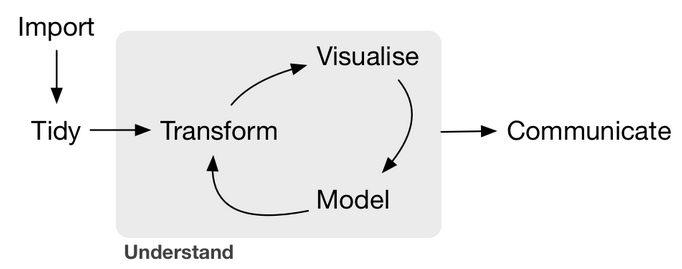
\includegraphics[width=0.75\textwidth]{../img/02_ciclo.png}
    \caption{Modelo de las herramientas que se necesitan en un proyecto de datos según \textcite[Introducción]{grolemund2016r}.}
    \label{fig:mesh1}
\end{figure}

\section{Importación de datos}\label{importacion-de-datos}

Para aplicar las herramientas de R a nuestro trabajo, es necesario poder
importar nuestros datos a R. R tiene conectores ya implementados para
casi cualquier tipo y formato de datos. Entre los más comunes están:

\begin{itemize}
\itemsep1pt\parskip0pt\parsep0pt
\item
  Archivos de texto plano (como csvs) con \texttt{readr}.
\item
  Datos desde una API con \texttt{httr}.
\item
  Binarios (como excel o sas) con \texttt{haven} y \texttt{readxl}.
\end{itemize}

\footnote{Los materiales para readr, httr, haven y readxl están basados en el capítulo de importación de datos de \textcite{grolemund2016r}.}

\section{Leer y escribir archivos de
datos}\label{leer-y-escribir-archivos-de-datos}

\subsection{Lectura}\label{lectura}

Desde archivo

Datos de muestra

\section{Extracción de partes de los
objetos}\label{extraccion-de-partes-de-los-objetos}

\subsection{Escritura}\label{escritura}

\section{Do's y don'ts de R}\label{dos-y-donts-de-r}

\subsection{Vectoriza y pre-asigna estructuras de
datos}\label{vectoriza-y-pre-asigna-estructuras-de-datos}

\subsection{Which}\label{which}

\subsection{La familia apply}\label{la-familia-apply}

\section{Dplyr}\label{dplyr}

La manipulación de datos es parte del ciclo de análisis de datos.

\begin{enumerate}
\def\labelenumi{\arabic{enumi}.}
\item
\end{enumerate}

\end{document}
